\clearpage

\subsection{例題9 四角形を描いてみる}

\subsubsection*{考え方}

四角形を描く命令、boxf命令を使ってみましょう。
まず簡単に背景の色を変えてみましょう。

\begin{description}
    \item color 255,255,255
    \item boxf
\end{description}

これで白い背景になります。

\begin{figure}[H]
    \begin{center}
        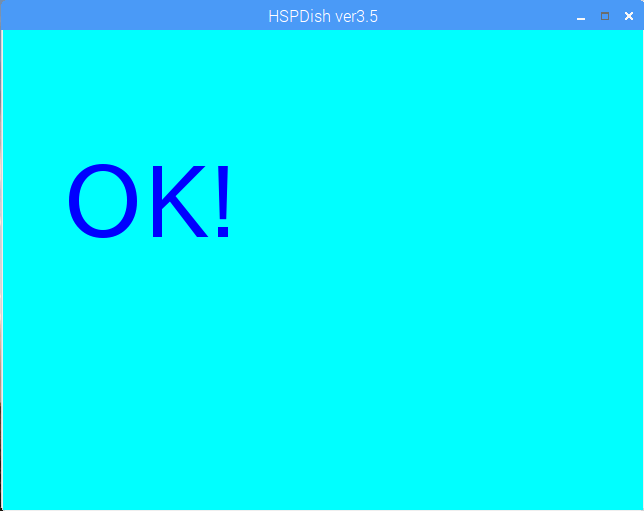
\includegraphics[keepaspectratio,width=6.006cm,height=4.77cm]{text02-img/text02-img036.png}
    \end{center}
\end{figure}

\begin{description}
    \item color 255,0,255
    \item boxf
\end{description}

のように修正すると色が変わります。

文字と同じようにcolor命令で四角形の色を変えることができます。

\begin{description}
    \item (例)
    \item boxf 100,200,200,250
\end{description}

パラメーターの数字4つを、増やしたり減らしたりしながら、四角形がどのように変わるか試してみましょう。

\subsubsection*{例題9 答え}

boxf命令は4つのパラメーターを指定します。

\begin{description}
    \item (HSPのルール)
\end{description}

\begin{description}
    \item 四角形を描くにはboxf命令を使います
    \item boxfの後はスペースに続けて4つの数字を指定します
    \item 4つの数字は「,」で区切ること
    \item 4つの数字は「左上横(よこ)の位置」「左上縦(たて)の位置」「右下横(よこ)の位置」「右下縦(たて)の位置」を指定する
    \item 4つのパラメーターを省略(しょうりゃく)すると全画面を塗りつぶします
\end{description}

実際に試してみて、四角形が描けたらTAや周りの友達にも見せてあげましょう。